\section{Lược đồ hoạt động}

\subsection{Activity Diagram cho Người dùng}

\subsubsection{Đăng ký}
\begin{figure}[H]
    \centering
    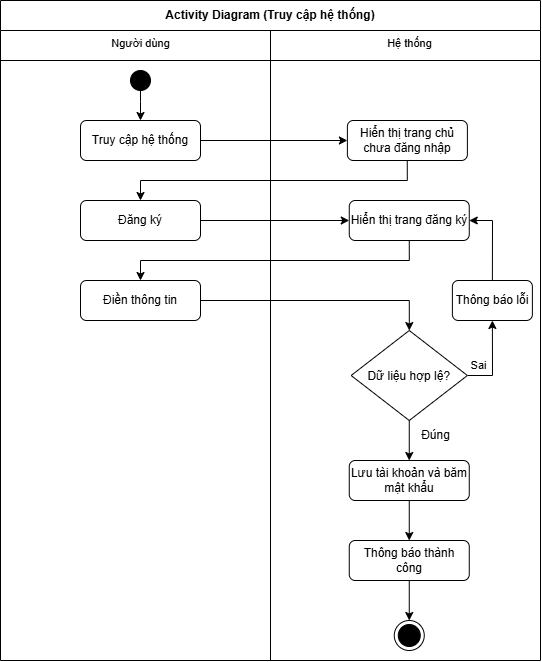
\includegraphics[width=0.7\textwidth]{Images/DangKy_ActivityDiagram.png}
    \vspace{15pt}
    \caption{Activity Diagram -- Đăng ký tài khoản}
\end{figure}

\indent \indent Người dùng chọn đăng kí tài khoản nếu chưa có tài khoản. Người dùng sẽ được chuyển hướng tới trang đăng kí. Sau khi người dùng nhập thông tin và chọn đăng kí, nếu
thông tin đã nhập là hợp lệ thì hệ thống sẽ lưu tài khoản và mã hóa mật khẩu. Trường hợp thông tin đã nhập được xác định là chưa hợp lệ, người dùng buộc phải nhập lại.


\subsubsection{Đăng nhập}
\begin{figure}[H]
    \centering
    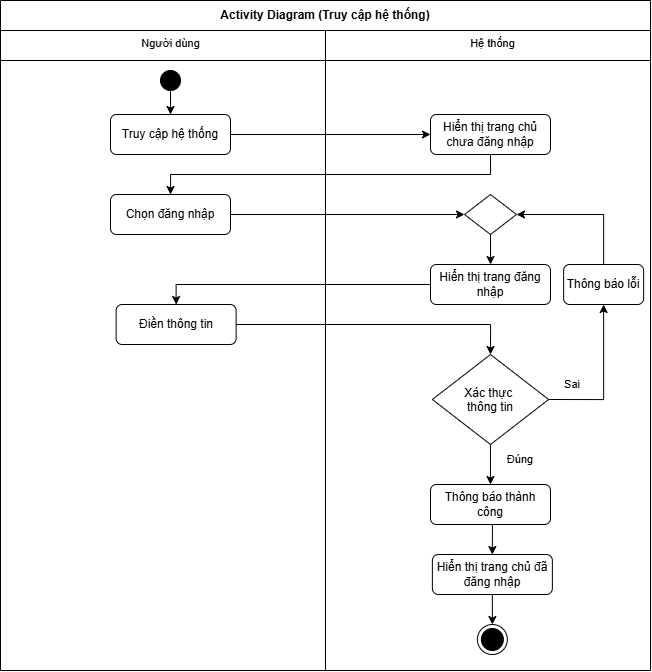
\includegraphics[width=0.7\textwidth]{Images/DangNhap_ActivityDiagram.png}
    \vspace{15pt}
    \caption{Activity Diagram -- Đăng nhập tài khoản}
\end{figure}

\indent \indent Người dùng sẽ nhập thông tin tài khoản để đăng nhập vào hệ thống. Sau khi đăng nhập thành công thì hệ thống sẽ chuyển hướng đến trang chủ. \\
\indent \underline{Lưu ý:} Sơ đồ hoạt động đăng nhập tài khoản trên có thể áp dụng cho cả Ban tổ chức hoặc quản trị viên trong cùng hoạt động.

\subsubsection{Mua vé sự kiện}

\begin{figure}[H]
    \centering
    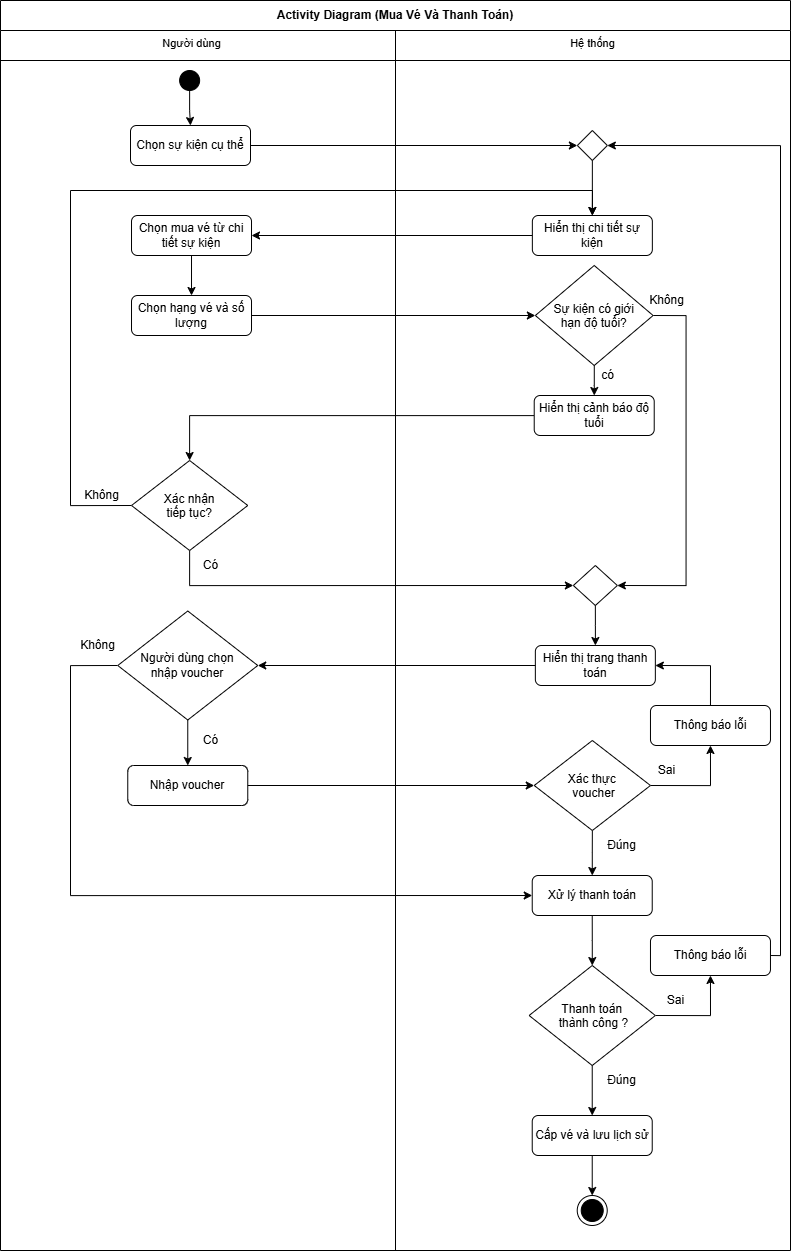
\includegraphics[width=0.7\textwidth]{Images/MuaVe_ActivityDiagram.png}
    \vspace{15pt}
    \caption{Activity Diagram -- Mua vé sự kiện}
\end{figure}

\subsubsection{Chat với Ban tổ chức hoặc quản trị viên}

\subsection{Activity Diagram cho Ban tổ chức}
\subsubsection{Đổi mật khẩu khi Ban tổ chức đăng nhập vào hệ thống lần đầu tiên}

\begin{figure}[H]
    \centering
    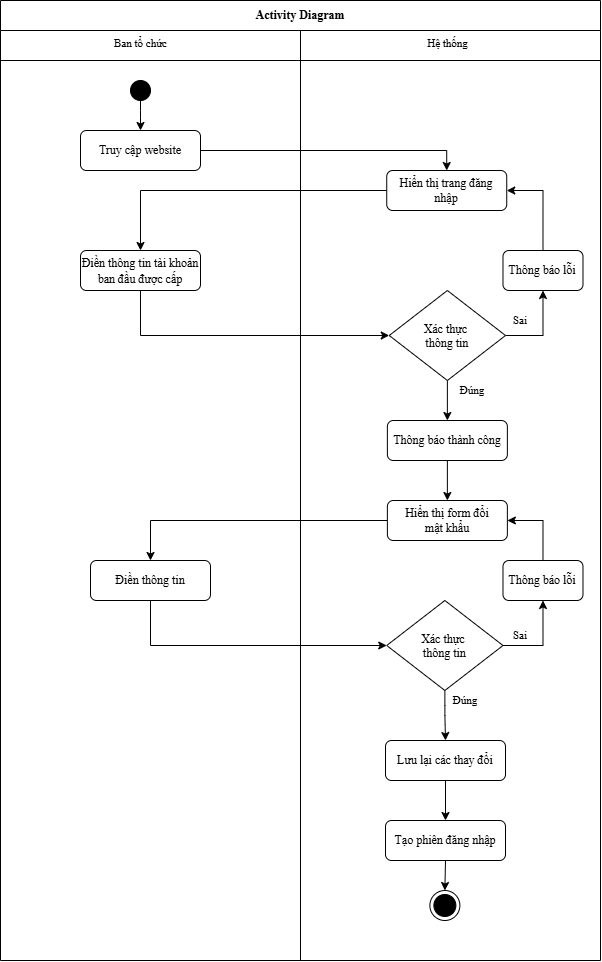
\includegraphics[width=0.7\textwidth]{Images/DoiMK_ActivityDiagram.png}
    \vspace{15pt}
    \caption{Activity Diagram -- Đổi mật khẩu trong lần đăng nhập đầu tiên}
\end{figure}

\indent \indent Khi đăng nhập thành công bằng tài khoản ban đầu được cấp, Ban tổ chức được chuyển hướng sang giao diện đổi mật khẩu để nhập các thông tin cần thiết. Trong trường hợp thông tin được nhập là hợp lệ, hệ thống sẽ lưu lại các thay đổi và tạo phiên đăng nhập. Nếu không, Ban tổ chức cần phải nhập lại các thông tin.

\subsubsection{Xem, tìm kiếm hoặc lọc danh sách sự kiện }
\begin{figure}[H]
    \centering
    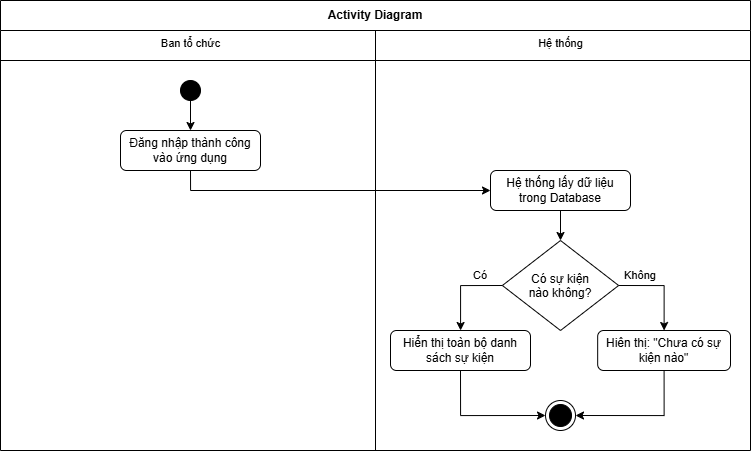
\includegraphics[width=0.7\textwidth]{Images/XemDSSK_ActivityDiagram.png}
    \vspace{15pt}
    \caption{Activity Diagram -- Xem danh sách sự kiện}
\end{figure}

\indent \indent Khi Ban tổ chức đăng nhập thành công, hệ thống sẽ hiển thị danh sách các sự kiện mà mình tổ chức đã được đăng tải lên hệ thống hoặc ngược lại sẽ trả về kết quả "Chưa có sự kiện nào".

\begin{figure}[H]
    \centering
    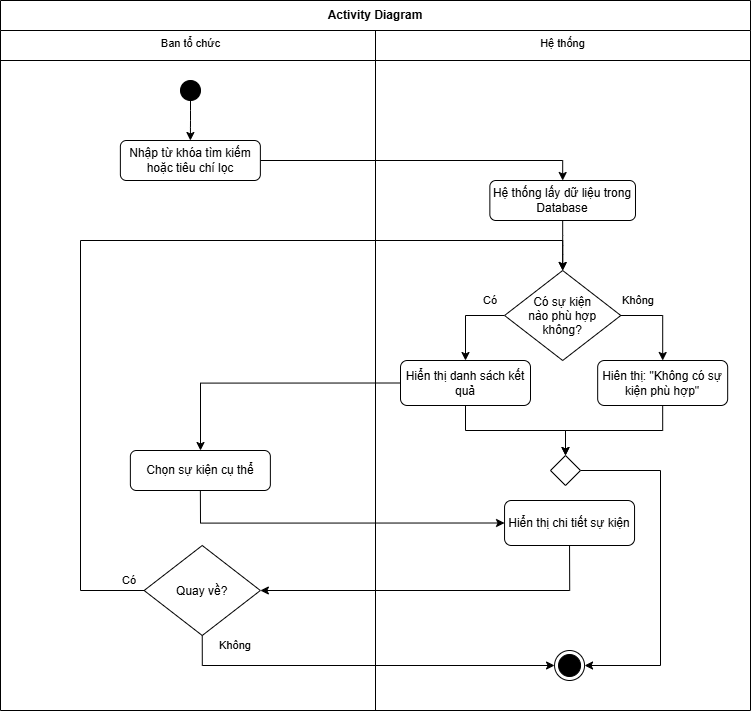
\includegraphics[width=0.7\textwidth]{Images/TimLocDSSK_ActivityDiagram.png}
    \vspace{15pt}
    \caption{Activity Diagram -- Tìm kiếm hoặc lọc danh sách sự kiện}
\end{figure}

\indent \indent Khi Ban tổ chức nhập từ khóa tìm kiếm hoặc chọn các tiêu chí lọc cụ thể, hệ thống sẽ hiển thi danh sách các sự kiện thỏa mãn hoặc ngoặc lại sẽ trả về kết quả "Không có sự kiện phù hợp". Trong trường hợp có sự kiện thỏa mãn, Ban tổ chức có thể nhấp vào 1 sự kiện cụ thể để xem chi tiết các thông tin liên quan.

\subsubsection{Phản hồi tin nhắn từ người dùng}

\begin{figure}[H]
    \centering
    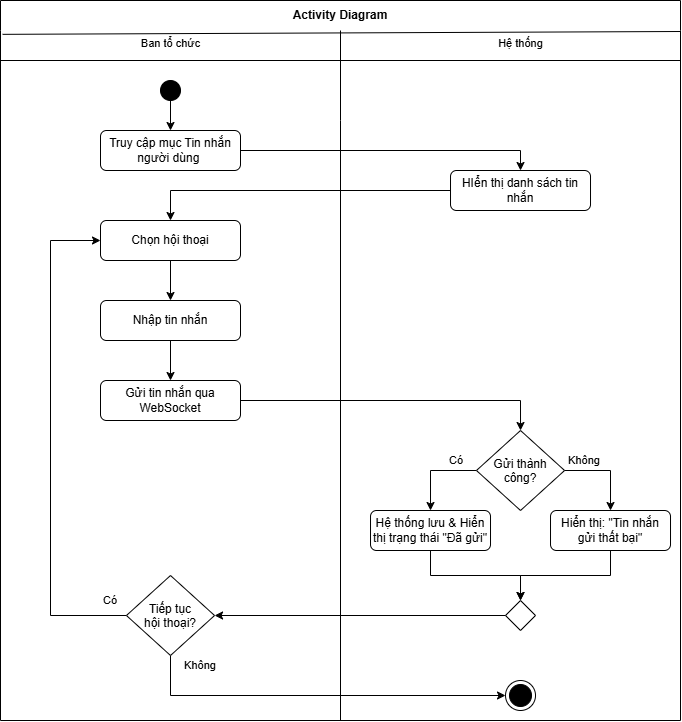
\includegraphics[width=0.7\textwidth]{Images/PhanHoiTinNhanNguoiDung_ActivityDiagram.png}
    \vspace{15pt}
    \caption{Activity Diagram -- Phản hồi tin nhắn từ người dùng}
\end{figure}

\indent \indent Ban tổ chức có thể xem các tin nhắn được gửi tới dựa trên danh sách tên người dùng (mục Tin nhắn từ người dùng). Để phản hồi, Ban tổ chức chọn người dùng cụ thể, nhập nội dung chat và nhắn gửi. \\
\indent \underline{Lưu ý:} Sơ đồ hoạt động phản hồi tin nhắn từ người dùng trên có thể áp dụng quản trị viên trong cùng hoạt động.

\subsection{Activity Diagram cho Quản trị viên}

\subsubsection{Quản lý danh sách các sự kiện}
\begin{figure}[H]
    \centering
    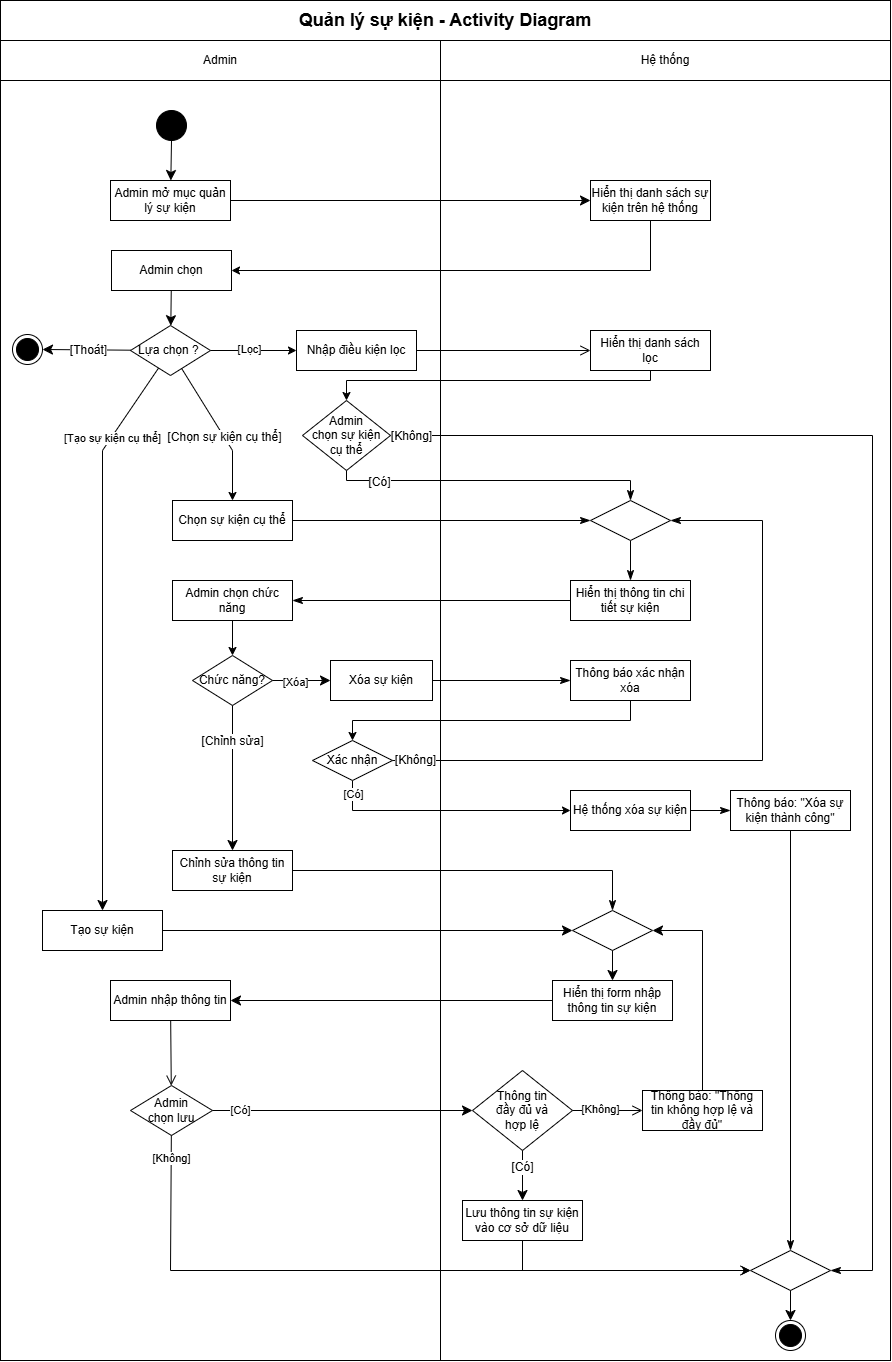
\includegraphics[width=0.7\textwidth]{Images/QuanLySuKien_ActivityDiagram.png}
    \vspace{15pt}
    \caption{Activity Diagram -- Quản lý danh sách sự kiện}
\end{figure}
\indent \indent Đầu tiên, admin mở mục quản lý sự kiện và có thể lọc hoặc chọn một sự kiện cụ thể để xem chi tiết. Từ đây, admin có thể thực hiện các chức năng như tạo mới, chỉnh sửa hoặc xóa sự kiện. Nếu xóa, hệ thống sẽ yêu cầu xác nhận và hiển thị thông báo sau khi xóa thành công; nếu chỉnh sửa hoặc tạo mới, hệ thống hiển thị form nhập liệu để admin điền thông tin. Sau khi admin lưu, hệ thống kiểm tra tính hợp lệ và đầy đủ của dữ liệu, rồi lưu thông tin vào cơ sở dữ liệu và thông báo kết quả tương ứng.
\subsubsection{Quản lý đơn vị tổ chức sự kiện}
\begin{figure}[H]
    \centering
    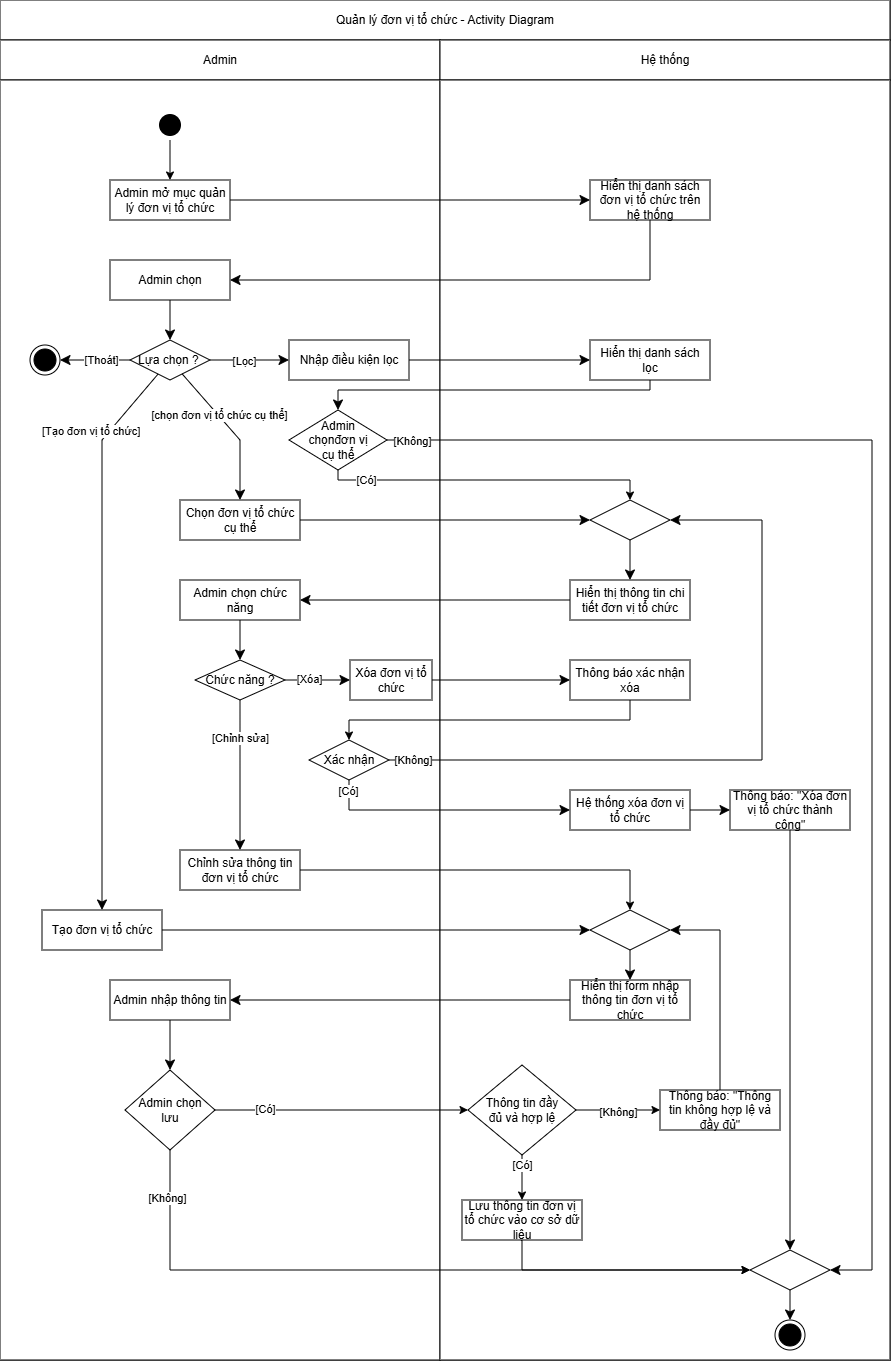
\includegraphics[width=0.7\textwidth]{Images/QuanLyToChuc_ActivityDiagram.png}
    \vspace{15pt}
    \caption{Activity Diagram -- Quản lý các đơn vị tổ chức sự kiện}
\end{figure}
\indent \indent Đầu tiên, admin truy cập mục quản lý và có thể thực hiện lọc danh sách hoặc chọn đơn vị cụ thể để xem chi tiết. Sau đó, admin có thể thực hiện các chức năng như tạo mới, chỉnh sửa hoặc xóa đơn vị tổ chức. Khi thực hiện thao tác xóa, hệ thống sẽ yêu cầu xác nhận trước khi xóa dữ liệu. Đối với thao tác thêm hoặc chỉnh sửa, hệ thống kiểm tra tính hợp lệ của thông tin và lưu vào cơ sở dữ liệu nếu hợp lệ, đồng thời hiển thị thông báo kết quả tương ứng.